\documentclass[tikz,border=10pt]{standalone}
\usepackage[utf8]{inputenc}
\usepackage[T1]{fontenc}
\usepackage[english]{babel}
\usepackage{graphicx}
\usepackage{amsmath,amssymb}
\usepackage{tikz}
\usepackage{hyperref}
\usepackage{geometry}
\usepackage{fancyhdr}
\usepackage{listings}
\usepackage{color}
\usepackage{caption}
\usepackage{booktabs}
\usepackage{longtable}
\usepackage{float}
\usepackage{array}
\usepackage{subfigure}
\usepackage{multirow}
\usepackage{multicol}
\usepackage[acronym]{glossaries}
\usepackage{xcolor}
\usetikzlibrary{shapes.geometric,arrows,positioning,calc,fit}

\begin{document}
\pagecolor{white}
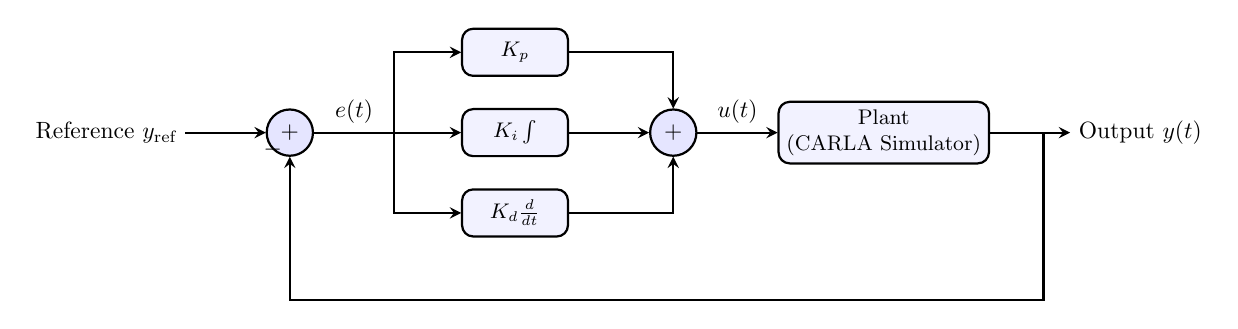
\begin{tikzpicture}[>=stealth, thick, scale=0.85, transform shape]
    \tikzset{
        block/.style={draw, fill=blue!5, rectangle, minimum height=2em, minimum width=4.5em, rounded corners, align=center, font=\small},
        sum/.style={draw, fill=blue!10, circle, minimum size=1.5em},
        line/.style={draw, ->, >=stealth, thick}
    }
    \node (ref) {Reference $y_{\text{ref}}$};
    \node [sum, right=1.2cm of ref] (sum) {$+$};
    \node [block, right=2.2cm of sum, yshift=1.2cm] (p) {$K_p$};
    \node [block, right=2.2cm of sum] (i) {$K_i \int$};
    \node [block, right=2.2cm of sum, yshift=-1.2cm] (d) {$K_d \frac{d}{dt}$};
    \node [sum, right=1.2cm of i] (sum2) {$+$};
    \node [block, right=1.2cm of sum2] (plant) {Plant\\(CARLA Simulator)};
    \node [right=1.2cm of plant] (out) {Output $y(t)$};
    
    \path [line] (ref) -- (sum);
    \coordinate (branch1) at ($(sum.east) + (1.2, 0)$);
    \draw [thick] (sum.east) -- node[above] {$e(t)$} (branch1);
    \path [line] (branch1) |- (p.west);
    \path [line] (branch1) -- (i.west);
    \path [line] (branch1) |- (d.west);
    
    \path [line] (p.east) -| (sum2);
    \path [line] (i.east) -- (sum2);
    \path [line] (d.east) -| (sum2);
    
    \path [line] (sum2) -- node[above] {$u(t)$} (plant);
    \path [line] (plant) -- (out);
    
    % Feedback loop
    \draw [line] (plant.east) -- +(0.8,0) |- +(0,-2.5) -| (sum.south);
    \node at (sum.south west) {$-$};
\end{tikzpicture}
\end{document}